\chapter{INTRODUCTION}

% \pagestyle{plain}

% no \PARstart
In recent years, wireless sensor networks (WSN) have become increasingly popular in playing the role of real world modalities. A WSN consists of a large number of tiny sensor nodes capable of interfacing with the real world, communicating wirelessly and performing limited computation. These tiny sensor nodes are low cost, low power and are easily deployable and can be readily networked and hence offers opportunity for a wide range of applications. Most popular areas for WSN applications are health, military, environment, home and security.
\section{Scope and Challenges}
\label{scope-challenges}
Due to tight integration with the physical world, sensor networks present significant challenges to the application development. As a result, most of the WSN applications till date focus on simple data-gathering and control designed to work on specific network and hence resulting in monolithic applications strongly coupled with protocols and network used. But as sensor network applications become pervasive, such monolithic and ad hoc approaches does not work and a systematic application design method based on standards and higher level abstractions is required \cite{Yu04}. To simplify sensor network application development, the need for programming abstractions such as a middleware framework is well acknowledged. WSN middleware can be considered as a software infrastructure that resides above operating system and below the application abstracting low-level functionality by providing high-level abstractions. A complete middleware solution should provide a holistic view of the network, services for data collection, aggregation and control while efficiently and adaptively managing system resources as per application's requirements. \\
% % % Resource management (DIRL+COIN)
WSN nodes are remarkably constrained in terms of their resources viz. energy, computational power and radio bandwidth. WSNs normally operate in uncertain and dynamic environments where the state of the system changes considerably over time. For example, in data collection applications, uncertainty exists due to intermittent links or traffic conditions. Moreover, the network itself is dynamic due to such events as node mobility and depleted battery. WSN applications need to cope with such dynamics and uncertainty inherent in sensor networks, while simultaneously trying to achieve application's requirements for QoS and optimization goal. Consequently, adaptive resource management is a key to any successful middleware solution enabling such applications.\\
Resource management includes initial sensor-selection and task allocation as well as runtime adaptation of allocated task/resources. There are many proposed middleware solutions that have advocated strong need for proactive adaptation of resources \cite{Heinzelman04,Marron05,Yu04}, but there are only few that have actually tried to resolve the issue of enabling adaptive resource management for WSN applications. This problem of resource management/adaptation (see Figure \ref{fig:res-management-problem}) can be described as follows: \\ 
\emph{Given application structure, QoS requirements and current system state, what is the
best way of allocating tasks to resources so that
given system-wide, application-driven, global
parameters can be optimized.}
%
\begin{figure}[tbp]
\centerline{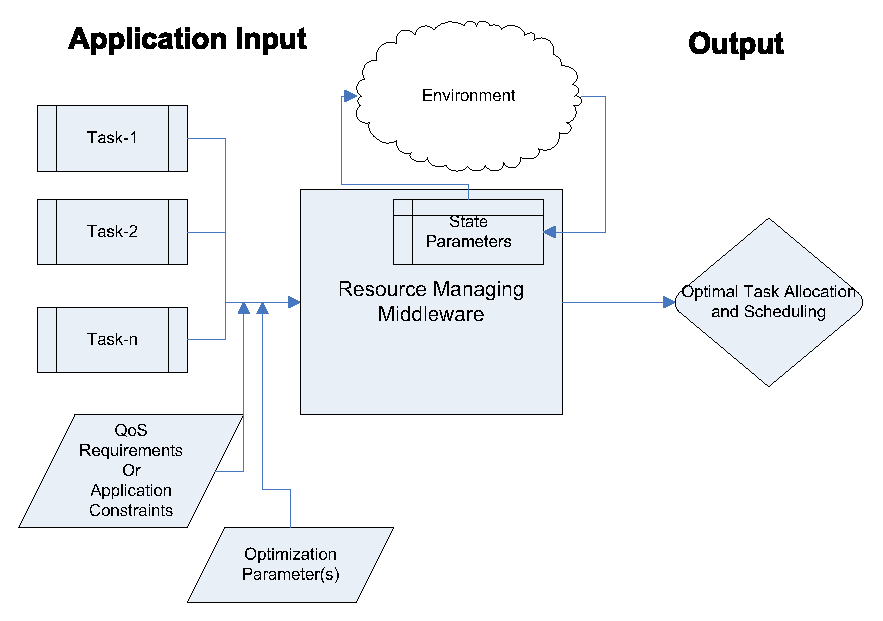
\includegraphics[width=4in]{figures/res-management-problem.eps}}
\caption{Resource management problem in WSN} 
\label{fig:res-management-problem}
\end{figure}
%
In the above, the application structure is in the form of underlying tasks and their interactions. QoS requirements include such constraints as latency, reliability, coverage etc. while the current state of the system is defined by parameters like mobility, energy availability, and neighboring nodes. The parameters to be optimized include energy, bandwidth, and network lifetime. Without loss of generality, we illustrate the resource management problem using a simplified object/entity tracking application (see Figure \ref{fig:res-management-intro}). Object tracking application can be considered to consist of following tasks: 1) sample- sense the environment (e.g. signal strength of a moving object). 2) transmit (Tx)- transmit a message to next hop towards the base-stations. 3) receive (Rx)- turn radio to receive mode to listen for incoming messages. 4) aggregate- aggregate two or more local and remote same target readings into single reading (e.g. data triangulation for better position estimation or mapping to a known track or simply \emph{last value} aggregation function). 5) sleep- put CPU and radio in sleep mode to minimize battery consumption. State representation may consist of the following variables: have one or more neighbors, successful in recent sampling, successful in recent receive, signal strength (or quality of reading). QoS requirements here may include quality of signal, tracking coverage area as well as maximum allowed latency. Our goal in this case is to optimize energy usage among all sensor nodes. Thus the goal of our resource management framework is to schedule and allocate tasks on each sensor node in the system, so that energy usage among all sensor nodes is minimized while fulfilling the coverage and latency requirements of the application.\\
\begin{figure}[tbp]
\centerline{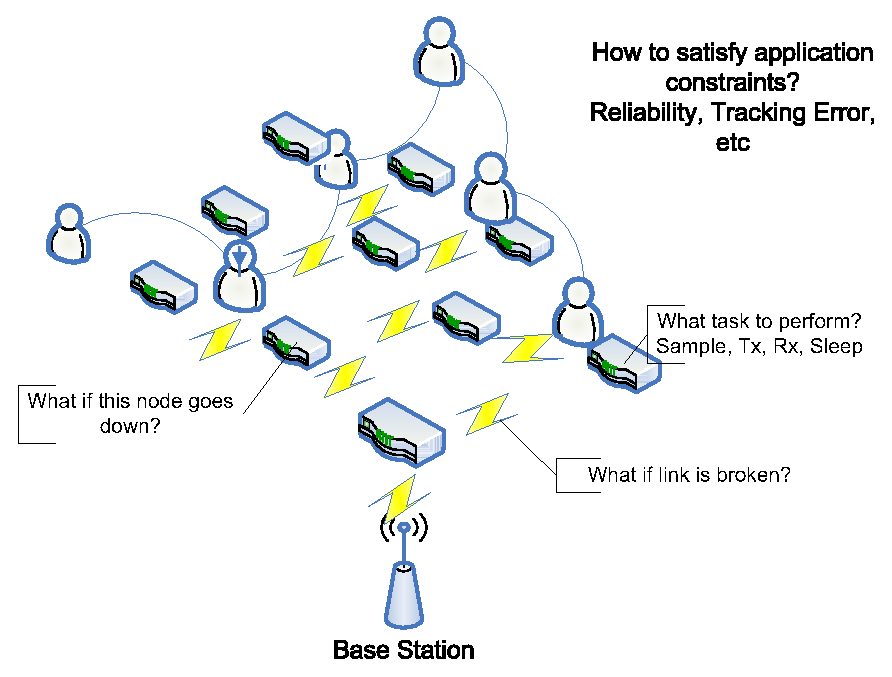
\includegraphics[width=4in]{figures/res-management-intro.eps}}
\caption{Resource management for object tracking application} 
\label{fig:res-management-intro}
\end{figure}
% % % Sparse WSN
Most sensor network applications studied today consists of a large number of sensor nodes deployed over a geographical area. Sensors use multi-hop communication to send data acquired from the external environment to a sink node or to an Access Point (AP) in the infrastructure. However, several applications do not require fine-grained sensing. Examples of such applications include monitoring of weather conditions in large areas, air quality in urban scenarios, terrain conditions for agriculture, and so on. In this case, it is possible to consider a \emph{sparse wireless sensor network}, i.e., a WSN where the density of nodes is so low that they cannot communicate with each other through multi-hop paths, or even directly. In order to make communication feasible, data collection in sparse WSNs can be accomplished by means of \emph{mobile data collectors} (MDCs). MDCs are special mobile nodes responsible for data gathering and/or dissemination. They are assumed to be powerful in terms of data storage and processing capabilities, and are not energy constrained. However, the data collection paradigm in sparse WSNs with MDCs is different, and introduces significant challenges including contact detection and energy conservation. \\
Communication between an MDC and each sensor node takes place in two phases. First, sensor node discovers the presence of the MDC in its communication range. Then, it transfers collected data to the MDC while satisfying any required reliability constraints. Unlike MDCs, sensor nodes have a limited energy budget, so that the data-collection process has to be energy efficient in order to prolong their network lifetime. In addition, such energy-conserving mechanisms should not compromise the timeliness of communication. This is critical especially when the MDC has only a short contact time with sensors, and also in the case when such contacts cannot be predicted accurately. In fact, a major problem in data collection is that sensor nodes usually do not have \emph{a priori} knowledge of the MDC mobility pattern. Furthermore, even in cases where the arrivals can be predicted, there is a chance that the MDC contacts can be affected by delays or can change their rate. Hence robust and flexible mechanisms have to be defined in order to adapt to operating conditions autonomously.\\ 
% % Communication Paradigm
Support for a scalable and robust communication paradigm is another important characteristic of a middleware solution. As all sensor network applications are data-driven, middleware should ideally support a data-centric model for task and data dissemination. Middleware should allow application specific in-network processing and data filtering to enable application assisted routing, aggregation, data fusion and collaborative information processing.
\section{Contributions}
\label{contributions}
We next introduce our contributions in this dissertation addressing the issues of developing a dynamic, adaptive and autonomous middleware for WSN management. 
% 
\subsection{Adaptive Resource Management Using Distributed Independent Reinforcement Learning}\label{intro:dirl}
Our first contribution is a Distributed Independent Reinforcement Learning (DIRL) based scheme for WSN resource management. The main idea of DIRL is to allow each individual sensor node to self-schedule its tasks and allocate its resources by learning their usefulness (utility) in any given state while honouring application defined constraints and maximizing total amount of reward over time. DIRL is based on Q-learning \cite{Watkins92}, a form of model-free reinforcement learning. Q-learning is quite simple, demands minimal computational resources and doesn�t require a model of the environment in order to operate. Hence it is ideal for implementation on resource-constrained sensor nodes. DIRL uses classic exploration and exploitation strategy as used in most RL based approaches to learn utilities of various tasks. DIRL addresses structural credit assignment (propagation of reward spatially across states in order to define notion of similar states) problem by using weighted hamming distance between two states. Here, the application state is represented in the form of system and application variables each carrying an associated weight. DIRL employs independent learning where each agent applies the learning algorithm in a classic sense (like single agent system) ignoring the presence of other agents. The main advantage of using independent learning in DIRL is that no communication is required for co-ordination between sensor nodes and each node selfishly tries to maximize its own rewards. 
% 
\subsection{Ensuring Global Optimization With Multi-Tier Reinforcement Learning}\label{intro:coin}
DIRL works well when each node in WSN application is acting of its own and doesn�t need to co-operate or compete with other nodes. In other words, if all nodes are acting independently and their actions do not affect others, then any increase in a node�s utility cannot decrease anyone else�s utility and hence will always increase world (system-wide) utility which is merely sum of all node�s utilities over all times. Such a system is sub-world factored and will eventually attain a Pareto-optimal point and hence towards our system-wide optimization goal. But most of the real-world WSN applications need some sort of co-operation among sensor nodes and hence nodes cannot work independently. In this case, increase in utility of individual node may result in reduction of other node�s utility and hence may not increase world utility. It is also possible that such system can lead to phenomena like Tragedy of the Commons (TOC) or Braes� Paradox, wherein individual�s selfishness leads to significantly lower world utility. Such phenomena can be avoided by carefully designing agent�s utility functions as well as constraints under which agent performs task selection. In other words, we need to make sure that individual�s utility is �aligned� with the world utility, i.e. any increase in agent�s private utility because of its action will also result in increase of world utility. COllective INtelligence (COIN) theory provides principles on designing such private (individual node) as well as global utility functions such that they are aligned. We follow these principles to design a multi-tier reinforcement learning based framework for WSN resource management.\\ 
Our design goal is to create a system using a bottom-up approach where each sensor node is responsible for task selection, rather than top-down approach (where some central entity dictates nodes what task to execute) used by many other middleware solutions [Heinzelman04, Yu04]. Main advantages of bottom-up approach are pro-active and real-time adaptation, no centralized processing requirement for task allocation and minimal communication overhead. But principal challenge of bottom-up approach is how to make sure that system is actually meeting the global application goals and is not just acting randomly or creating chaos. We resolve this issue by using two-layer learning: micro-learning as used by individual nodes to self-schedule their tasks and macro-learning as used by each data-stream subworld to steer the system towards application goal by setting/updating rewards for micro-learners. 
%
\subsection{Resource-aware Data Collection in Sparse Wireless Sensor Networks}\label{intro:dirl-sparse}
Next we explore the issue of energy-aware resource allocation in sparse WSNs with Mobile Data Collectors (MDCs). We define discovery and data transfer protocols for energy-efficient data collection in sparse WSNs with MDCs, and propose an adaptive strategy exploiting our Distributed Independent Reinforcement Learning scheme. We design a generic adaptive data collection (ADC) framework that can be applied to wide range of applications while minimizing energy consumption. The principal idea is to learn underlying pattern of MDCs' arrival and tune sensor node's duty cycle accordingly. Through extensive simulations, we show that our framework is highly efficient in terms of low duty cycle, high discovery rate and high energy and data transfer efficiency.
%
\subsection{Design of Adaptive Middleware Using Directed Diffusion}\label{intro:diffusion}
%
\section{Organization of Dissertation}\label{organization}
In chapter 2, we review existing literature and provide some necessary background on a few related topics that have been used in this dissertation. Chapter 3 describes our preliminary DIRL scheme for resource management in WSN. We present our extended multi-tier reinforcement learning based framework using COIN and DIRL in Chapter 4. In chapter 5, we explore application of DIRL to sparse WSN for energy-aware MDC discovery. Chapter 6 provides a detail design of our complete adaptive and autonomous middleware.